\documentclass[conference]{IEEEtran}
\usepackage{graphicx}
\usepackage{tikz}
\usepackage{caption}
 
\usepackage[colorlinks = true, citecolor = blue]{hyperref}

% math lib
\usepackage{amsmath}
\usepackage{mathrsfs}

% operators
\DeclareMathOperator*{\argmax}{arg\,max}
\DeclareMathOperator*{\argmin}{arg\,min}
\newcommand\ceiling[1]{\left\lceil #1 \right\rceil}

% empty set
\usepackage{amssymb}
\let\emptyset=\varnothing

% algorithms
\usepackage{algorithm}
\usepackage{algorithmic}
\renewcommand{\algorithmicrequire}{\textbf{Input:}}
\renewcommand{\algorithmicensure}{\textbf{Output:}}

\begin{document}
% --------------------------------------------
% --------------Change HERE! -----------------
% --------------------------------------------
\def\authorone{Jonathan Jiang}
\def\authortwo{Tiantong Li}
\def\groupid{8}
% --------------------------------------------
\title{CS258 Final Report: The RSA Problem}
\author{
    \IEEEauthorblockN{\authorone\ and \authortwo}
    \IEEEauthorblockA{
        Group \groupid
    }    
}

\maketitle
\IEEEpeerreviewmaketitle


\section{Methods: RL-based Routing}
\subsection{RL Algorithms}
% List RL algorithms and give a brief explanation of each
In the project, two RL algorithms were used. The first one is Proximal Policy Optimization (PPO). And the second one is Asynchronous Proximal Policy Optimization (APPO). 

PPO is a reinforcement learning algorithm developed by OpenAI, a family of policy optimization methods that use multiple epochs of stochastic gradient ascent to perform each policy update \cite{schulman2017proximal}. PPO offers some of the advantages of Trust Region Policy Optimization (TRPO), but they are much simpler to implement, more general, and have better sample complexity.

APPO is an asynchronous variant of Proximal Policy Optimization (PPO) based on the IMPALA architecture. This is similar to IMPALA but uses a surrogate policy loss with clipping. In IMPALA, a central learner runs SGD in a tight loop while asynchronously pulling sample batches from many actor processes \cite{raydocument}.

Compared to synchronous PPO, APPO is more efficient in wall-clock time due to its use of asynchronous sampling. Using a clipped loss also allows for multiple SGD passes, and therefore the potential for better sample efficiency compared to IMPALA.

In the project, we experimented with both RL algorithms, and the difference in the results are shown and analyzed in \ref{sec:util} and \ref{sec:comparison}.




\subsection{State Space}
The state represents the current status of the environment that our agent finds itself in at any given time.

An example of a state in our project would be the link states. At a given round time 
T, the link states, defined by the number of colors currently occupied in our graph, represent the current status of our graph.

However, to manage the graph effectively, we also have the EdgeState class from A4. These EdgeState instances contain information about the colors and requests, including holding time, source, and destination, that are currently occupied for each edge. This information is crucial and can be used to reconstruct the entire graph. Additionally, we maintain a self.\textunderscore round\textunderscore to\textunderscore EdgeStats list that contains EdgeState instances for each round.

These pieces of information can be used to construct the graph at any given round time, allowing us to calculate the utilization of each edge at any given time.

\subsection{Action Space}

The action represents the current choices made by the agent that affect the state of the environment. Actions are selected based on the algorithm of our reinforcement learning model.

In the project, an action would be one of the possible paths that an agent can choose to route its request. For example, if there are two paths between nodes 1 and 7: (1,2,0,7) and (1,3,0,4,7), then these two paths correspond to action 0 and action 1.

To define the action spaces for this experiment, the Dijkstra algorithm is used to find the shortest path between nodes. After obtaining the shortest distance between nodes, a Depth-First Search algorithm is used to obtain all possible paths between nodes where the length of the paths is one more or equal to the shortest path.

\subsection{Reward Function}
An example of a reward would be the feedback from our current routing action. If a request is successfully routed in the graph, then a positive reward is returned since the action achieved a desired outcome. However, if the request is not successfully routed or it picks a wrong action (for example, in case 2, choosing a path that does not connect the source and destination of the request), a negative reward would be given, indicating a poor choice was made.


\section{Method: Spectrum Allocation}
% Explain your heuristic
% If you have multiple, you can make subsections 
For spectrum allocation, the same method in A4 was adopted, which uses the shortest path and index-based allocation. One adjustment made was that instead of one single shortest path, two paths between the source (San Diego Supercomputer Center) and destination (Jon Von Neumann Center, Princeton, NJ) could be used by the requests. The first one is (7, 0, 2, 1) and the second one is (7, 6, 12, 4, 1). These two paths combined utilize 7 edges in the network, which consists of 15 edges in total. Since the 100 requests are all trying to leave from San Diego to Jon Von Neumann Center, and the capacity of each edge is 10, a great number of blocks were observed. 

\section{Results}
\subsection{Learning Curve}
% Insert figures
% Explain the results
Learning curves are utilized to assess whether the agent effectively learns through reinforcement algorithms. The following learning curves are created by TensorBoard, and they represents the relationship between rewards and episodes. 

In Fig \ref{fig:LcPPO}, the learning curve of PPO has shown that the reward is increasing over time, which means the agent can learn to make better decisions. The algorithm is run over 800 rounds, 32000 episodes, with a learning rate of 0.001.


In Fig \ref{fig:APPOreward}, the learning curve of APPO has shown that the reward keeps fluctuating, which means the agent isn't able to learn to make better decisions to increase the reward over time. The algorithm is run over 800 rounds, 32000 episodes, with a learning rate of 0.001.

\begin{figure}[h]
    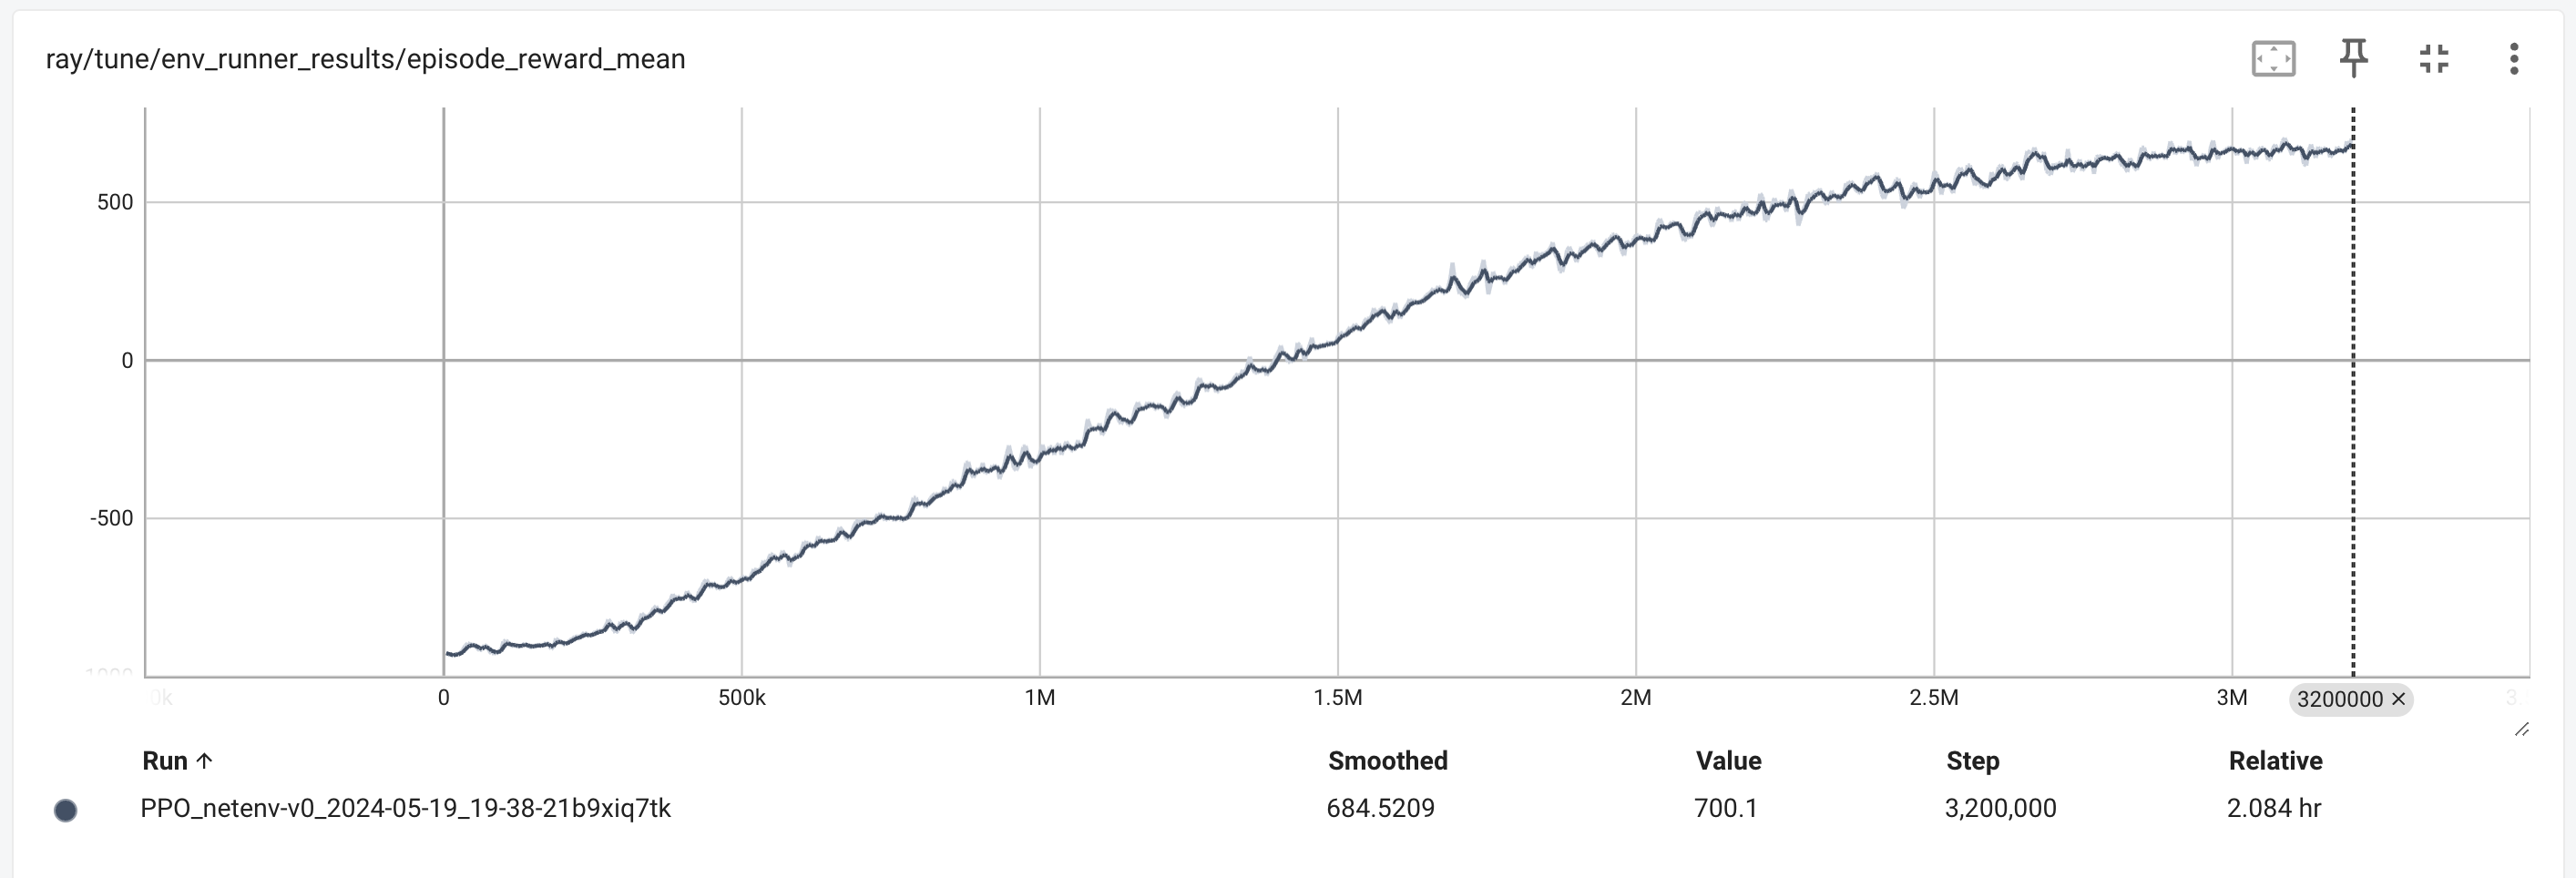
\includegraphics[width=0.48\textwidth]{learning_curve_PPO.png}
    \caption{Learning curve of PPO in Case 2}
    \label{fig:LcPPO}
\end{figure}

\begin{figure}[h]
    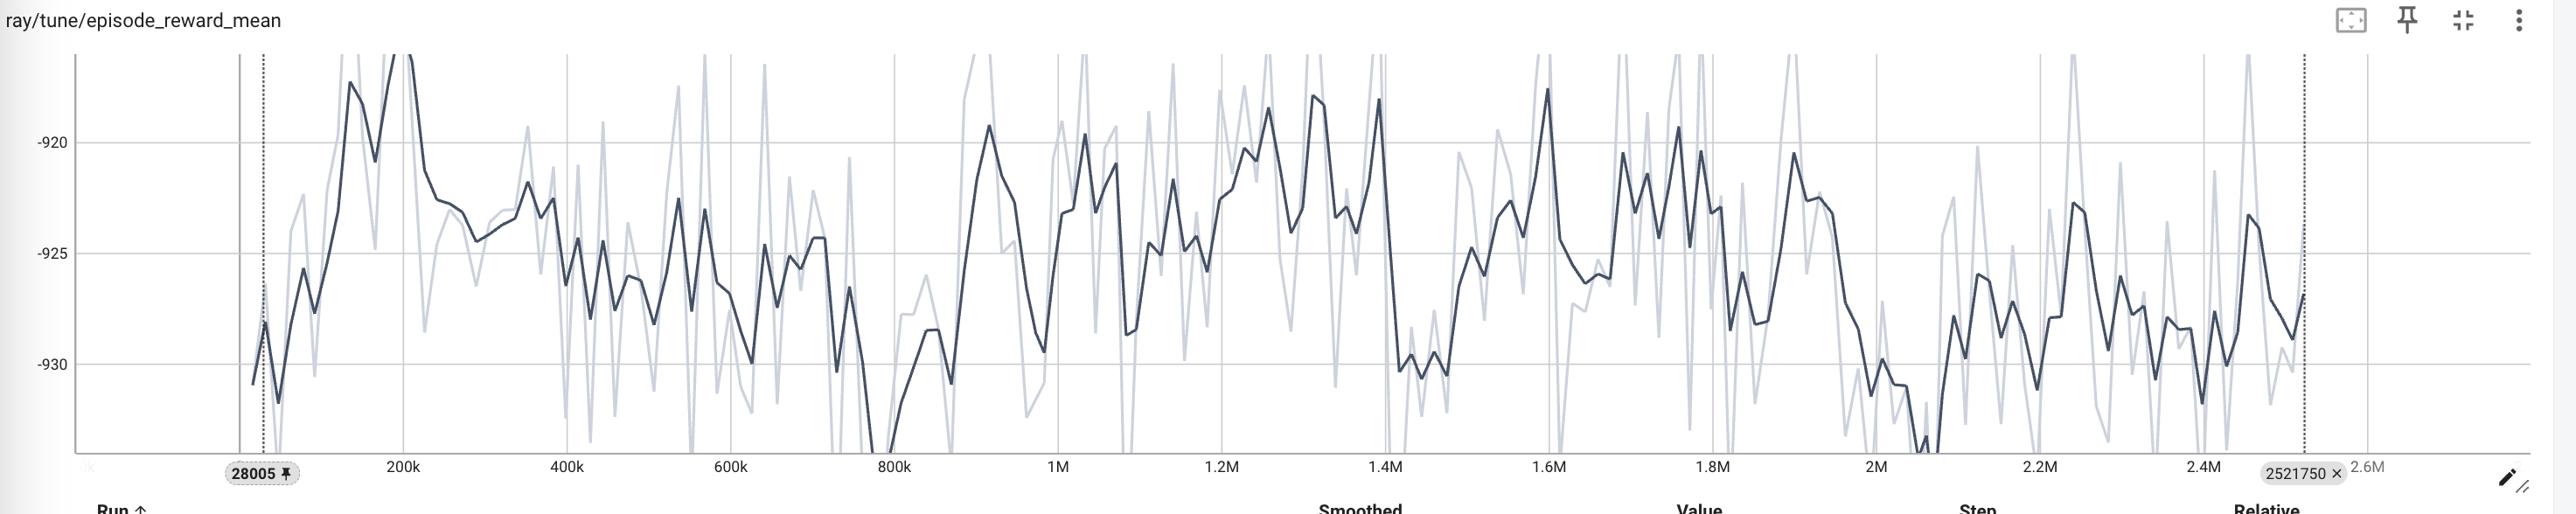
\includegraphics[width=0.48\textwidth]{appo_reward_mean.png}
    \caption{Learning curve of APPO in Case 2}
    \label{fig:APPOreward}
\end{figure}

\subsection{Utilization (The Objective)}
\label{sec:util}

Let \(c_{t,e}\) denote the capacity of a link \( e\) at time \( t\) and \(o_{t,e}\) represent the occupied slots of a link \(e\) at a time \( t \), then the utilization  of the link  at a time  can be computed by:
\[
u_{t,e} = \frac{o_{t,e}}{c_{t,e}}
\]

The average utilization of a link \( U_{e} \) of \(e\) over \(T\) episodes is:
\[
 U_{e} = \frac{1}{T} \sum_{t=0}^{T-1} u_{t,e}
\]

The network-wide utilization is defined as the average of the edge total utility:
\[
\text{Utilization} = \frac{1}{|E|} \sum_{l \in E} \overline{U}_l
\]

The objective function is the network-wide utilization over time and our goal is to maximize the objective function.

% % 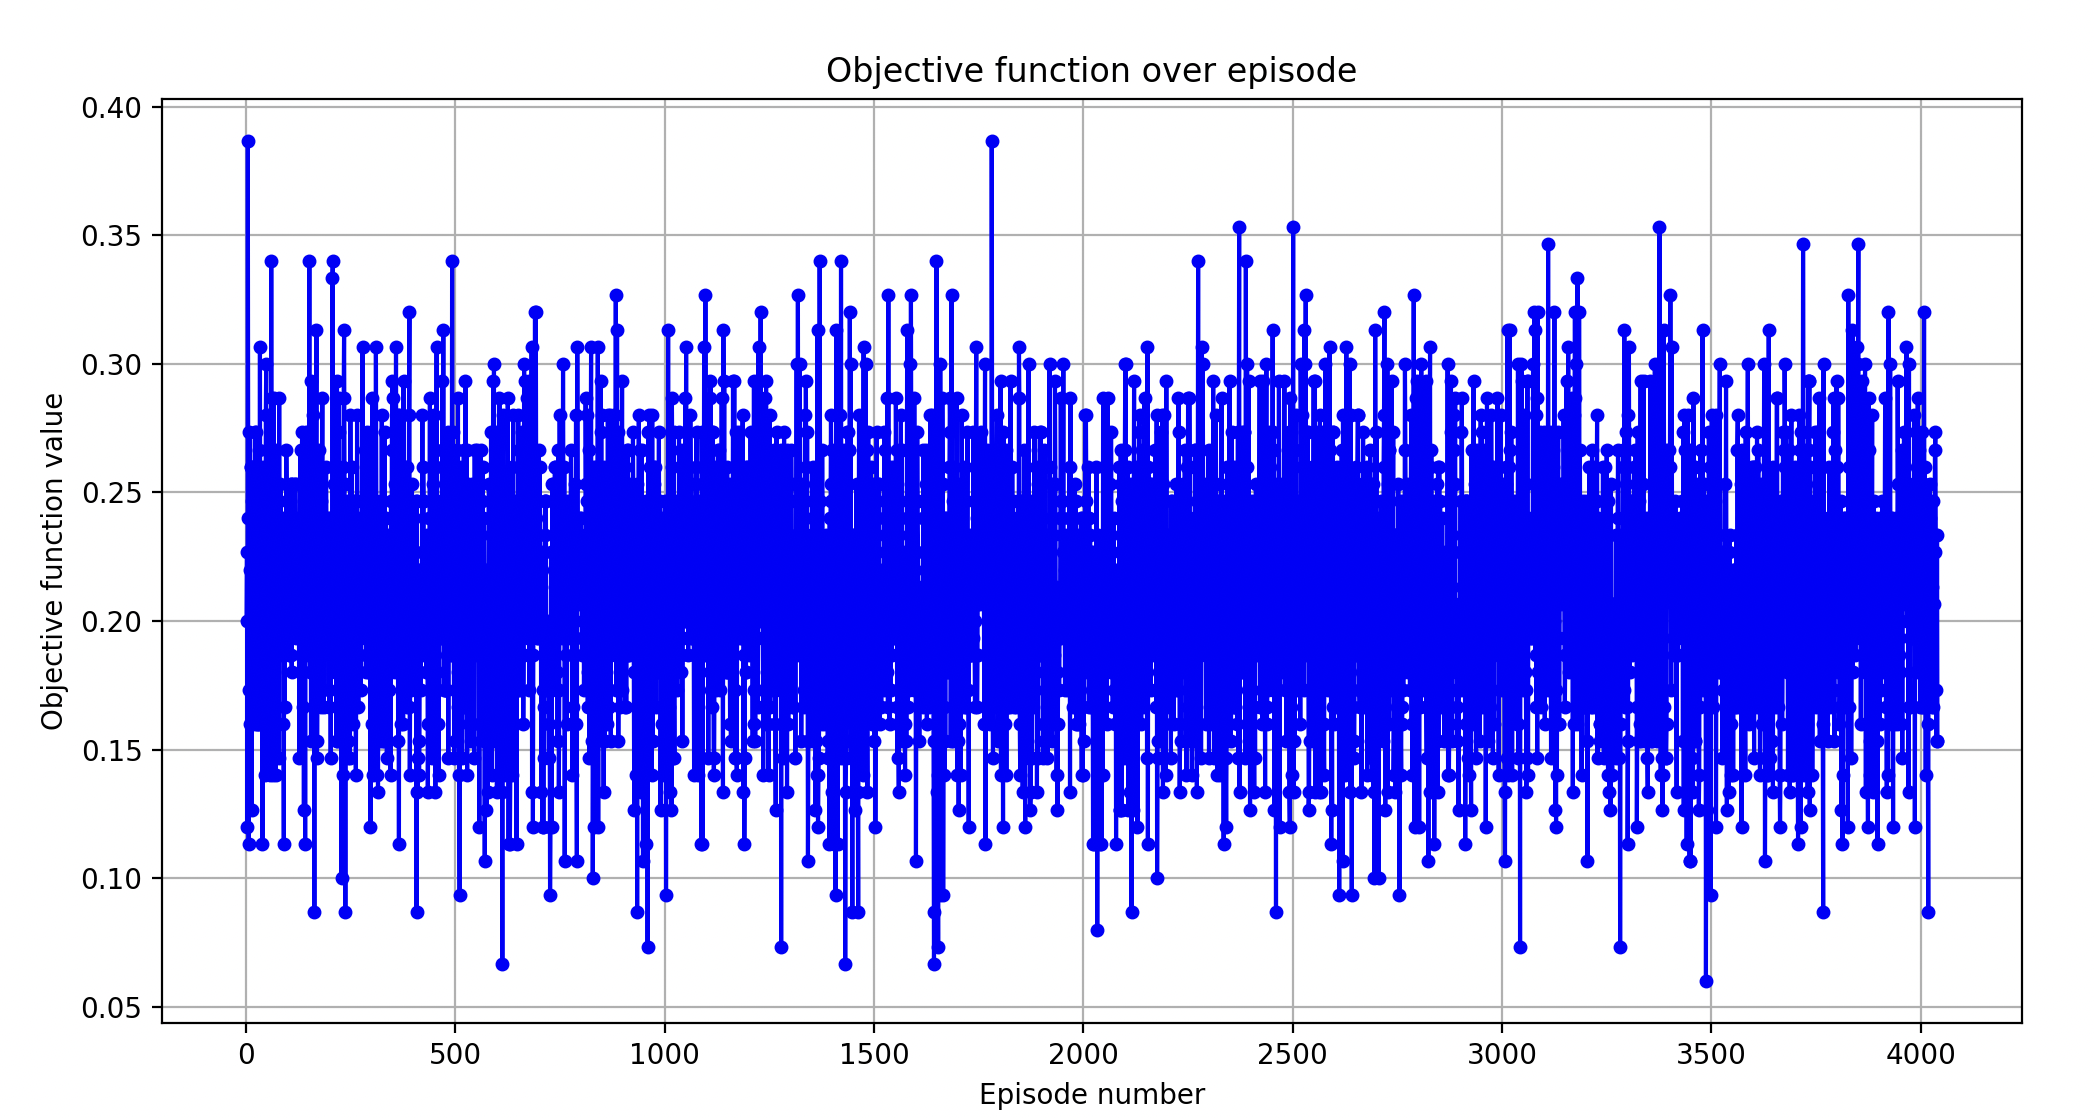
\includegraphics[width=0.5\textwidth]{case1.png}

In Fig \ref{fig:case1}, the objective function of Case 1 fluctuates between around 0.05 and 0.4.

\begin{figure}[h]
    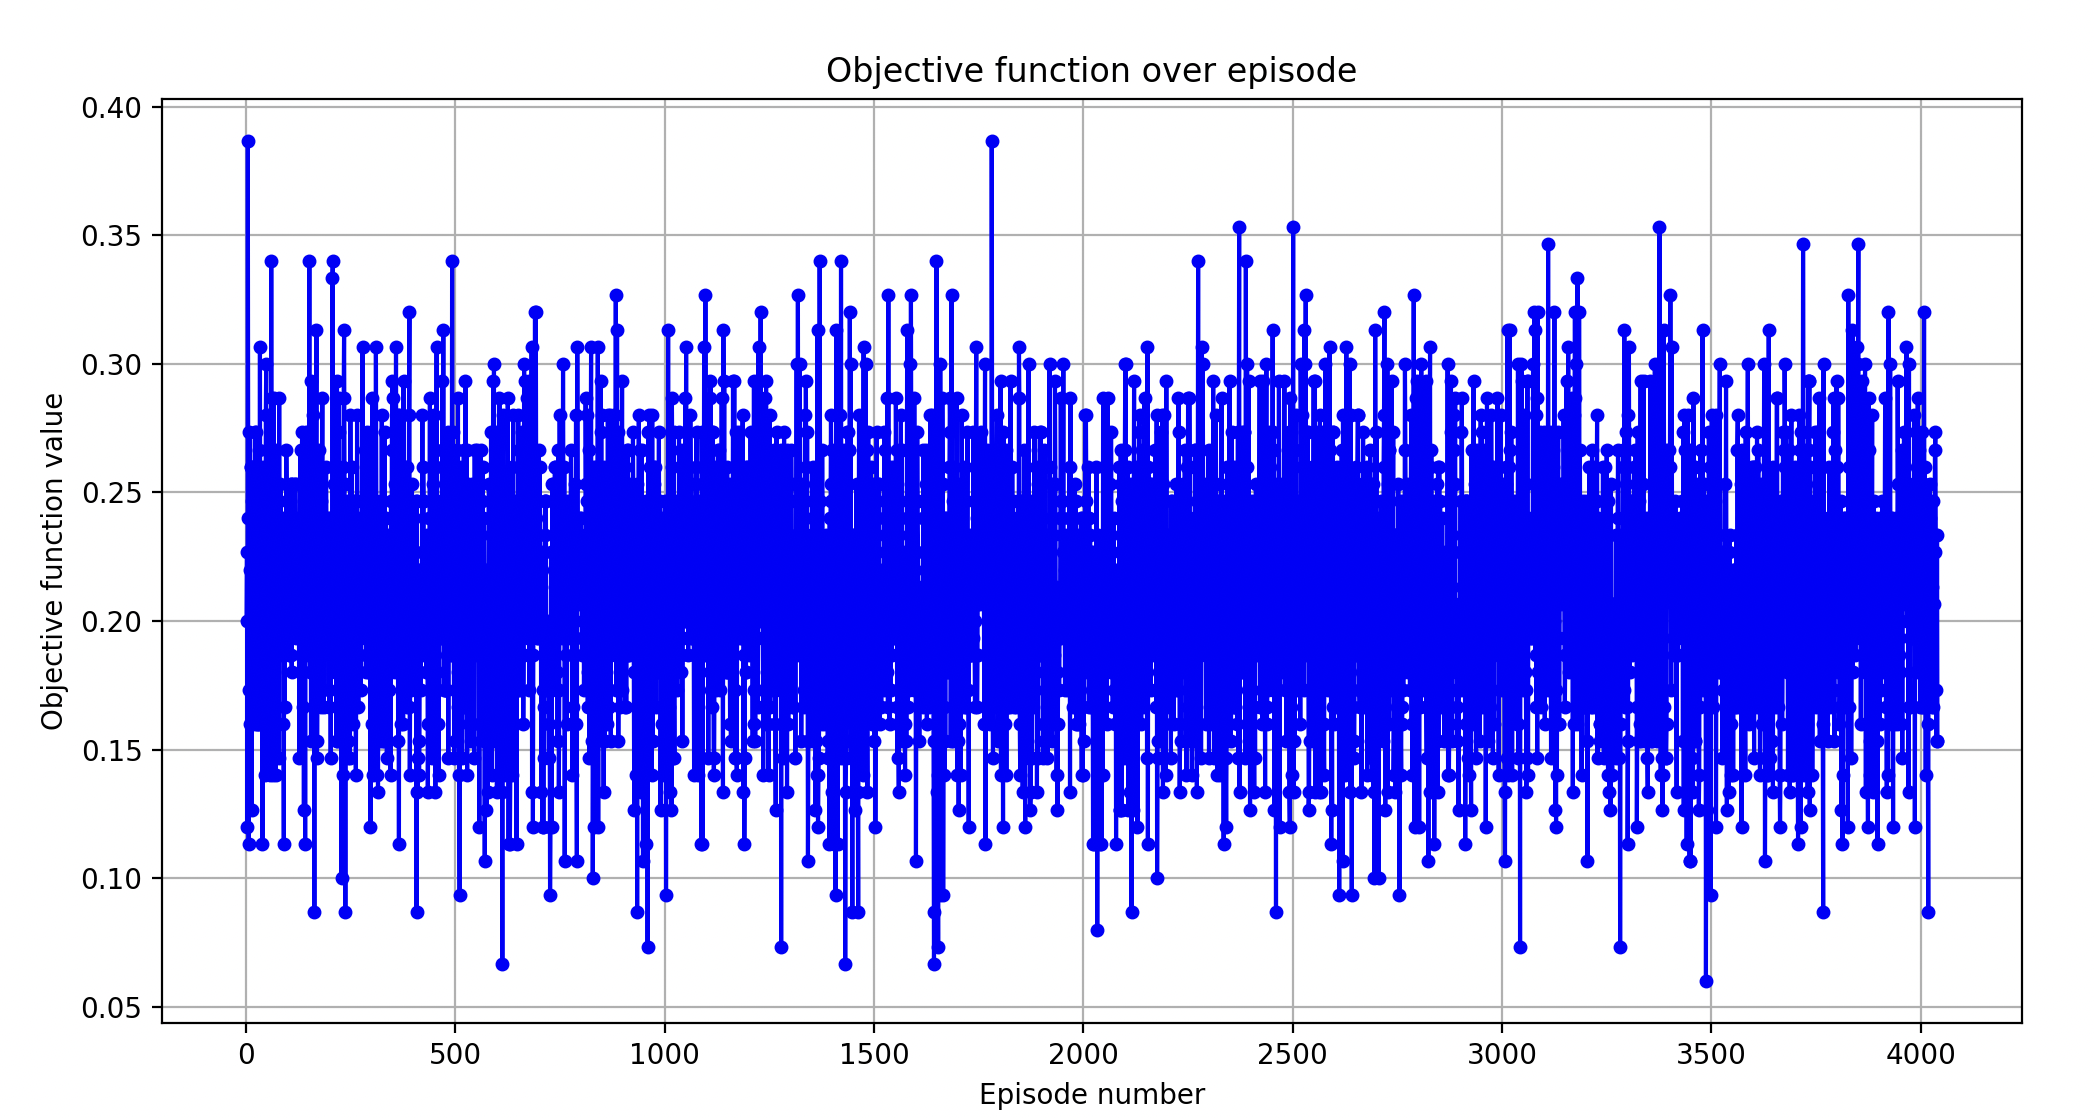
\includegraphics[width=0.48\textwidth]{case1.png}
    \caption{Objective function of Case 1}
    \label{fig:case1}
\end{figure}

In Fig \ref{fig:PPOcase2}, the objective function of PPO in Case 2 is over 32000 episodes. The maximum objective function is 0.12. As there are objective function as low as 0.0 over time, in the last 100 episodes, only 4 objective functions return 0, while in the first 100 episodes, 92 objective functions return 0. 


\begin{figure}[h]
    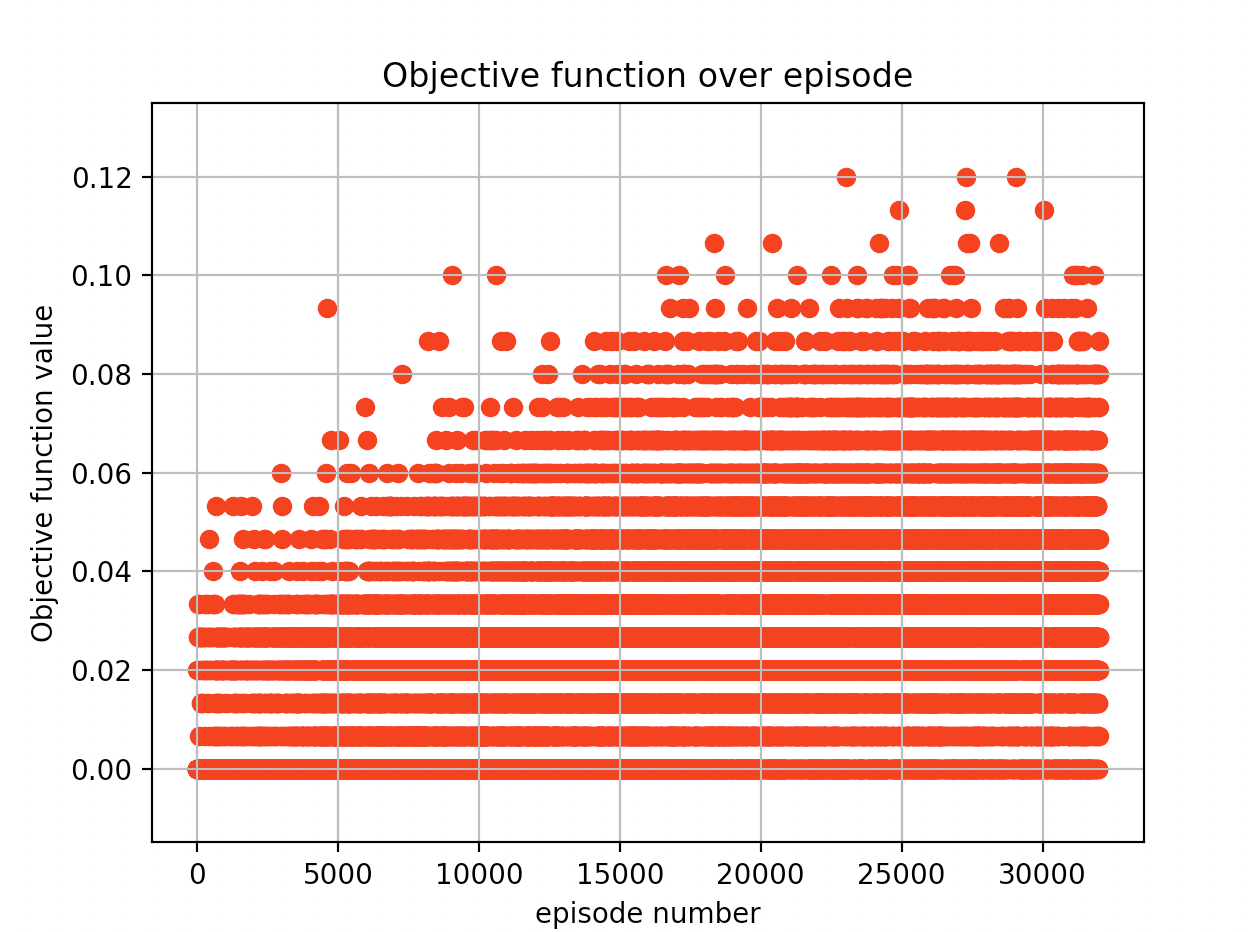
\includegraphics[width=0.48\textwidth]{case2_PPO_objec_func.png}
    \caption{Objective function of PPO in Case 2}
    \label{fig:PPOcase2}
\end{figure}


In Fig \ref{fig:APPOcase2}, the objective function of APPO in Case 2 was assessed across 32000 episodes. While the maximum value reached 0.053, there were instances where it dropped as low as 0.0 over time. These findings suggest that the APPO algorithm isn't performing satisfactorily for our project, as the graph doesn't exhibit a consistent upward trend in the objective function. This is also reflected in the learning curve (Fig \ref{fig:APPOreward}), where rewards aren't increasing as the number of episodes progresses. This observation suggests a potential failure in the learning process.


\begin{figure}[h]
    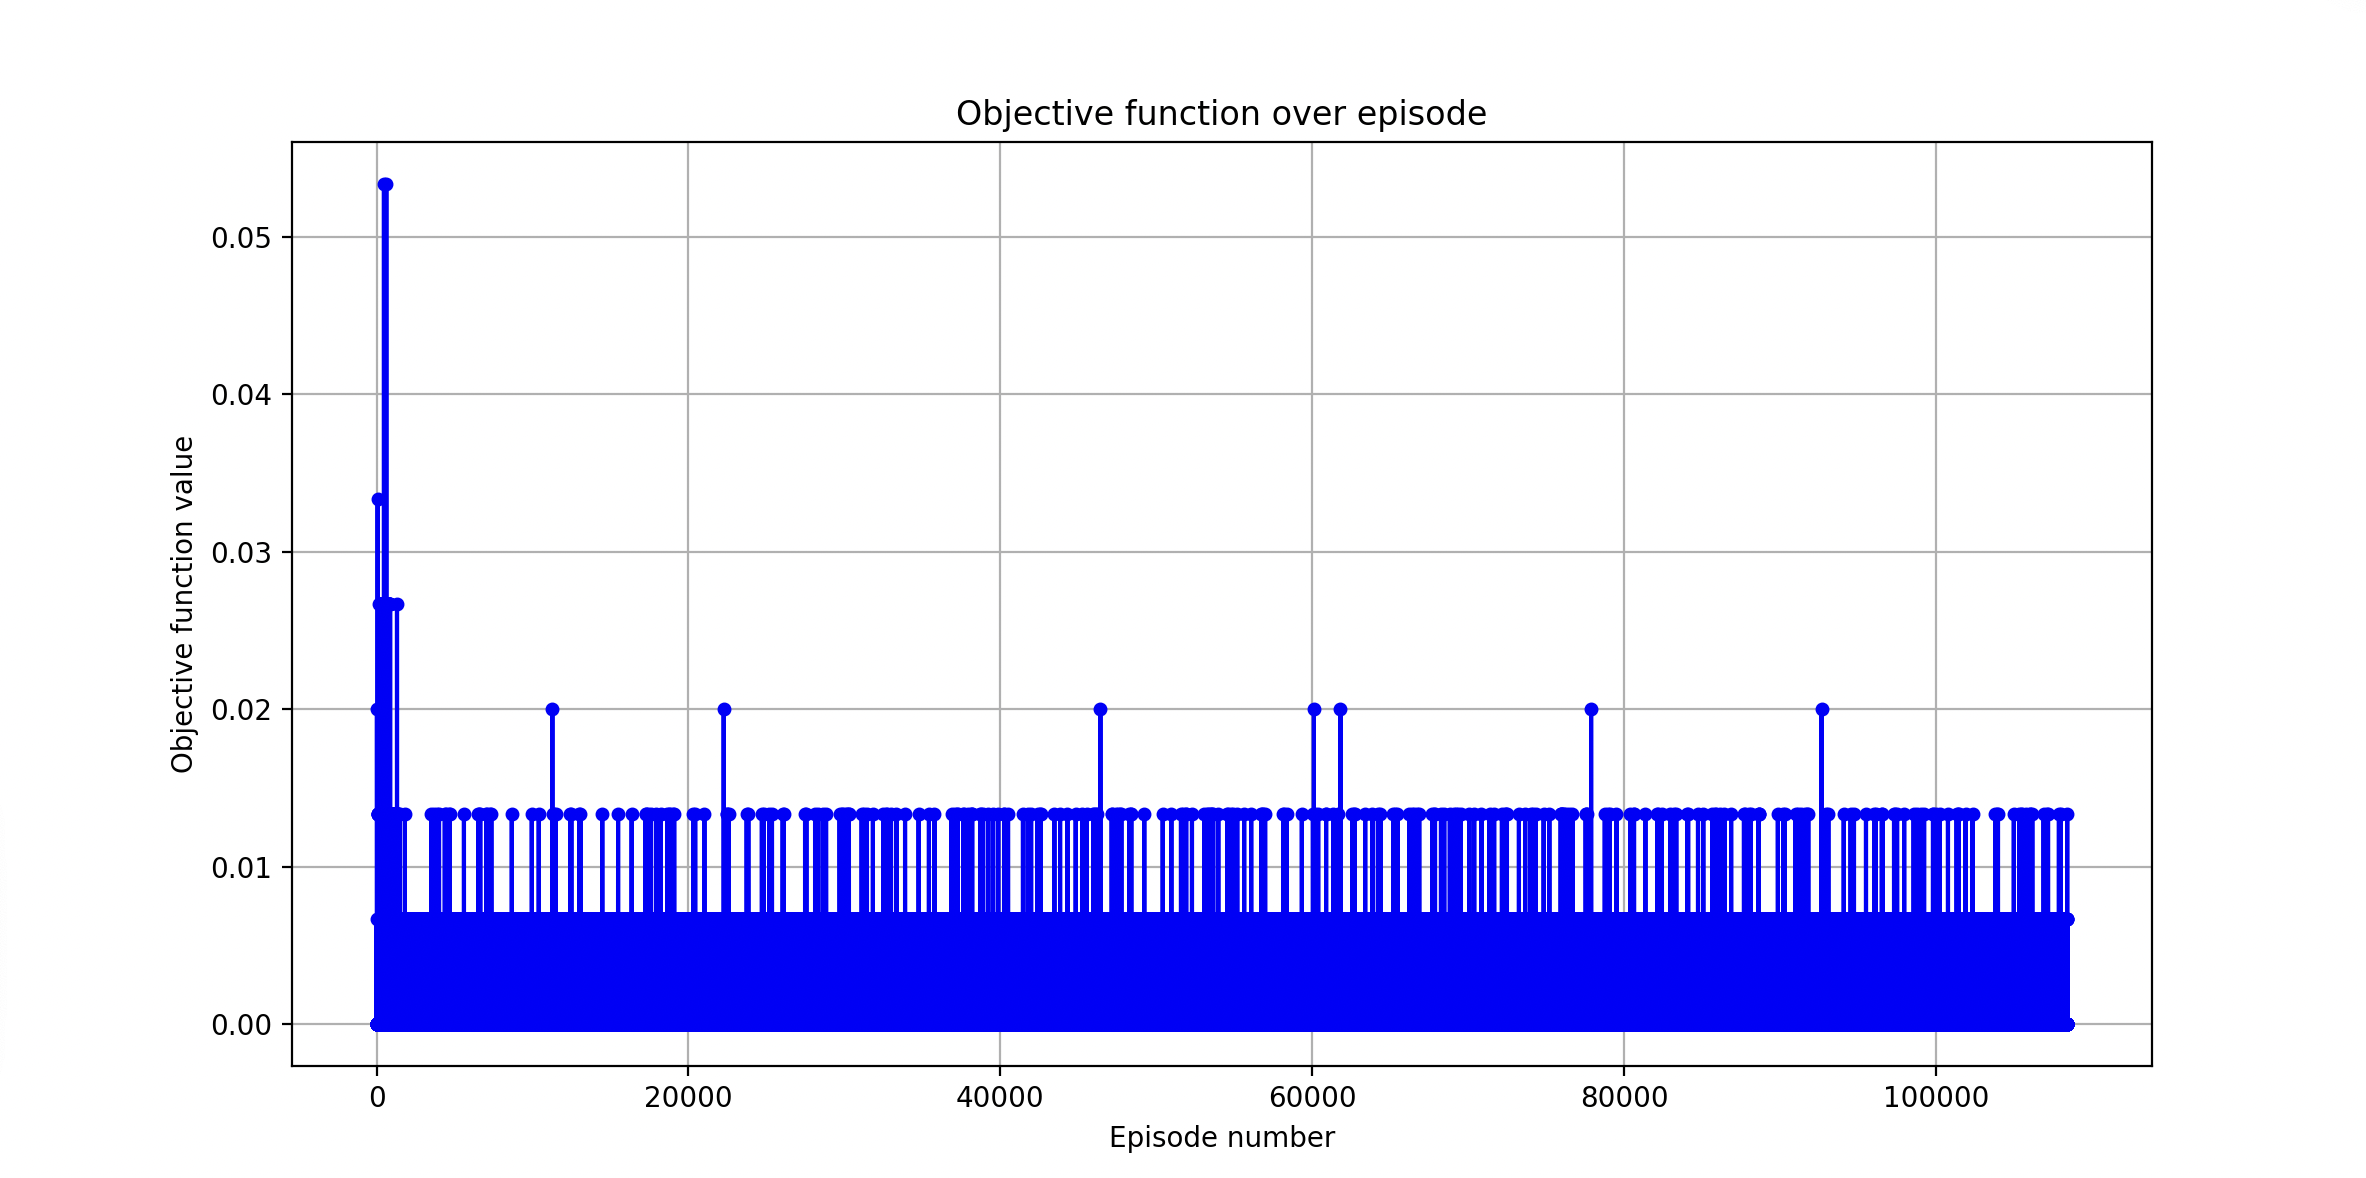
\includegraphics[width=0.48\textwidth]{case2_APPO_objec_func.png}
    \caption{Objective function of APPO in Case 2}
    \label{fig:APPOcase2}
\end{figure}

\subsection{Comparison}
\label{sec:comparison}
The comparison between the two objective functions reveals that the PPO algorithm consistently outperforms APPO. Furthermore, among the three routing strategies evaluated, PPO generates the most superior routing solutions over time. This is evidenced by the positive correlation between its learning curve and the objective function. This experiment has provided valuable insights into the application of reinforcement learning techniques for solving routing problems.


\bibliography{ref}


\bibliographystyle{ieeetr}


\end{document}
